% =====================================================================
%  Coordinate Provenance
%
%  Self-contained. Every construction used is defined here; no companion
%  paper is required. External citations are to the mass spectrometry,
%  graph theory, and measurement literature only.
% =====================================================================
\documentclass[11pt,a4paper]{article}

\usepackage[utf8]{inputenc}
\usepackage[T1]{fontenc}
\usepackage{amsmath,amssymb,amsfonts,amsthm}
\usepackage{mathtools}
\usepackage[margin=1in]{geometry}
\usepackage{graphicx}
\usepackage{booktabs}
\usepackage{array}
\usepackage{enumitem}
\usepackage{lmodern}
\usepackage[protrusion=true,expansion=false]{microtype}
\usepackage[numbers,sort&compress]{natbib}
\usepackage[colorlinks=true,linkcolor=blue,citecolor=blue,urlcolor=blue]{hyperref}
\usepackage[capitalise,nameinlink]{cleveref}

% ---------------------------------------------------------------------
%  Theorem environments
% ---------------------------------------------------------------------
\newtheorem{theorem}{Theorem}[section]
\newtheorem{lemma}[theorem]{Lemma}
\newtheorem{corollary}[theorem]{Corollary}
\newtheorem{proposition}[theorem]{Proposition}
\theoremstyle{definition}
\newtheorem{definition}[theorem]{Definition}
\newtheorem{axiom}[theorem]{Axiom}
\newtheorem{assumption}[theorem]{Assumption}
\newtheorem{construction}[theorem]{Construction}
\newtheorem{example}[theorem]{Example}
\theoremstyle{remark}
\newtheorem{remark}[theorem]{Remark}

% ---------------------------------------------------------------------
%  Notation
% ---------------------------------------------------------------------
\newcommand{\Obs}{\mathcal{O}}               % observation set
\newcommand{\Crd}{\mathcal{K}}               % coordinate space
\newcommand{\Ctx}{\mathcal{C}}               % context space
\newcommand{\Prv}{\mathcal{P}}               % provenance record
\newcommand{\aud}{\mathrm{aud}}
\newcommand{\rec}{\mathrm{rec}}
\newcommand{\adr}{\mathrm{addr}}
\newcommand{\dep}{\delta}
\newcommand{\flo}{\beta}
\newcommand{\resid}{R}
\DeclareMathOperator*{\argmin}{arg\,min}
\DeclareMathOperator*{\argmax}{arg\,max}

\title{\textbf{Coordinate Provenance:\\[2pt]
Auditing Derived Coordinates in Analytical Pipelines}}

\author{Kundai Farai Sachikonye\\
\texttt{kundai.sachikonye@wzw.tum.de}}

\date{\today}

\begin{document}
\maketitle

% =====================================================================
\begin{abstract}
\noindent
Analytical pipelines increasingly index measurements not by their raw
quantities but by derived coordinates: normalised scores, embedded
vectors, hierarchical addresses, confidence triples. A coordinate is
convenient precisely because it discards the context in which it was
computed, and that is also what makes it unauditable. We formalise the
problem. A coordinate map sends a measurement together with a context ---
calibration state, reference set, tuning parameters, software version ---
to a point in a coordinate space, and the coordinate alone does not
determine the context. We prove that this is not a shortcoming of any
particular map but a counting fact: any coordinate map onto a space
smaller than its context-augmented domain is non-injective in the
context argument, so distinct contexts collapse onto identical
coordinates (\Cref{thm:collapse}). We prove that the collapse is
transitive under composition, so a pipeline of coordinate stages loses
auditability monotonically (\Cref{thm:pipeline-loss}), and that no
downstream stage recovers it (\Cref{cor:no-recovery}). The positive
results follow. We define a \emph{provenance-carrying coordinate} as a
pair of a coordinate and a record, give the minimal record sufficient for
re-derivation (\Cref{thm:minimal-record}), prove that carrying it costs
storage linear in the number of stages rather than in the number of
measurements (\Cref{prop:cost}), and prove that a
provenance-carrying pipeline admits a decision procedure for whether two
coordinates are comparable at all (\Cref{thm:comparability}). We show
that comparability failure is common and silent in practice: two
normalised intensities from different runs, two hierarchical addresses
built at different depths, two confidence scores from differently tuned
models. The recommendation is an interface: coordinates should be typed
by their context, comparison should be a partial operation that declines
when the types differ, and pipelines should expose a re-derivation
function rather than a provenance log.
\end{abstract}

% =====================================================================
\section{Introduction}
\label{sec:intro}

Raw mass spectrometry data is a list of $(m/z, \text{intensity},
\text{time})$ triples. Almost nothing downstream operates on it directly.
Instead the pipeline computes coordinates: retention time is converted to
an index normalised against standards, intensity is converted to a
relative abundance normalised against a reference channel, spectral
similarity is converted to a score against a library, a candidate
identification is converted to a confidence value, and a feature is
assigned an address in a hierarchical index for retrieval. Each of these
is a coordinate in the sense used here: a value computed from a
measurement and something else.

The something else is the difficulty. A normalised retention index is
meaningless without knowing which standards were used. A relative
abundance is meaningless without knowing which channel is the reference.
A library score is meaningless without knowing the library version, its
preprocessing, and the scoring function's parameters. Yet the coordinate
is a single number, and by the time it reaches the analysis that consumes
it, the standards, the reference, and the library version are typically
recorded in a log file if they are recorded at all.

This is not a plea for better logging. Logging is necessary and does not
suffice, for a reason this paper makes precise: a log records what was
done, but comparability is a property of pairs of coordinates, and
establishing it requires deciding whether two records agree in the
respects that matter for the comparison at hand. A log answers ``what
happened''; the question is ``may I subtract these two numbers''. The
second does not reduce to the first without a formal account of what a
coordinate depends on.

\subsection{The problem, concretely}

Two laboratories report the retention index of a compound as $1247$. In
the first, the index is normalised against a homologous series of
$n$-alkanes; in the second, against a series of alkyl esters. The
numbers are equal. They are not comparable, because equality of
coordinates in different coordinate systems carries no information
\citep{vandendool1963generalization,krokhin2006sequence}. Nothing in
either number reveals the discrepancy, and an analysis that pools the two
values produces a well-formed result that means nothing.

The same structure recurs at every stage. Two relative abundances of
$0.63$ from differently referenced channels. Two spectral match scores of
$0.91$ from differently versioned libraries. Two hierarchical addresses
that agree in their first three symbols but were constructed to different
depths, so that agreement at depth three means ``indistinguishable'' in
one and ``distinguished but truncated'' in the other. In each case, the
coordinate is a valid output of a correct computation, and the comparison
is invalid.

\subsection{What is proved}

\Cref{sec:setting} formalises coordinate maps as functions of a
measurement and a context. \Cref{sec:collapse} proves the negative
results: context collapse is forced by counting (\Cref{thm:collapse}),
compounds under composition (\Cref{thm:pipeline-loss}), and is not
recoverable downstream (\Cref{cor:no-recovery}). \Cref{sec:record}
gives the positive construction: provenance-carrying coordinates, the
minimal sufficient record (\Cref{thm:minimal-record}), and its cost
(\Cref{prop:cost}). \Cref{sec:comparability} proves the decision
procedure for comparability (\Cref{thm:comparability}) and shows that
declining is the correct output when it fails
(\Cref{thm:decline-sound}). \Cref{sec:floor} establishes that the record
cannot be compressed to nothing --- there is a positive floor on what
must be carried (\Cref{thm:record-floor}). \Cref{sec:practice} applies
the results and states the interface.

% =====================================================================
\section{Setting}
\label{sec:setting}

\begin{definition}[Measurement and context]\label{def:meas}
Let $X$ be a finite set of \emph{measurements} --- the possible raw
values a stage can receive --- and $\Ctx$ a finite set of \emph{contexts}.
A context is everything the stage consults other than the measurement:
calibration standards, reference channels, library versions, tuning
parameters, and the software revision that implements the stage.
\end{definition}

Finiteness of $\Ctx$ is not restrictive. Any context realised in a
laboratory is specified by finitely many finitely-representable choices;
the set of contexts that ever occur is finite, and only that set matters
below.

\begin{definition}[Coordinate map]\label{def:coord}
A \emph{coordinate map} is a function $\varphi : X \times \Ctx \to \Crd$
into a \emph{coordinate space} $\Crd$. We write
$\varphi_c(x) = \varphi(x,c)$ for the map at fixed context.
\end{definition}

\begin{example}[Instances]\label{ex:instances}
Retention index: $X$ is elution times, $\Ctx$ is the choice of standard
series and its calibration table, $\Crd \subseteq \mathbb{R}$. Relative
abundance: $X$ is a raw intensity, $\Ctx$ is the reference channel and
its normalisation constant, $\Crd = [0,\infty)$. Library score: $X$ is a
spectrum, $\Ctx$ is the library and scoring parameters, $\Crd = [0,1]$.
Hierarchical address: $X$ is a feature vector, $\Ctx$ is the alphabet,
the discretisation thresholds, and the depth, $\Crd = \Sigma^{\leq k}$.
\end{example}

\begin{definition}[Auditability]\label{def:audit}
A coordinate map $\varphi$ is \emph{auditable} if there exists
$\aud : \Crd \to \Ctx$ with $\aud(\varphi(x,c)) = c$ for all
$x \in X$, $c \in \Ctx$; that is, if the context can be read off the
coordinate.
\end{definition}

\begin{definition}[Comparability]\label{def:comparable}
Two coordinates $k_1,k_2 \in \Crd$ produced by $\varphi$ are
\emph{comparable} if there exist $x_1,x_2$ and a \emph{single} context
$c$ with $k_i = \varphi(x_i,c)$. Otherwise they are \emph{incomparable}.
\end{definition}

\Cref{def:comparable} is the operative notion. It says that a comparison
between coordinates is licensed exactly when the two coordinates could
have arisen in one and the same context; arithmetic on coordinates
computed in different contexts is arithmetic on values that were never
on a common scale.

% =====================================================================
\section{Context Collapse}
\label{sec:collapse}

\begin{theorem}[Collapse is forced]\label{thm:collapse}
If $|\Crd| < |X| \cdot |\Ctx|$ then $\varphi$ is not injective, and if
moreover $|\Crd| < |\Ctx|$ for some fixed $x$ with $\varphi(x,\cdot)$
considered alone, there exist $c_1 \neq c_2$ with
$\varphi(x,c_1) = \varphi(x,c_2)$. In either case $\varphi$ is not
auditable in the sense of \Cref{def:audit} unless $\varphi$ is injective
in its second argument for every fixed first argument.
\end{theorem}

\begin{proof}
The first claim is the pigeonhole principle applied to
$\varphi : X \times \Ctx \to \Crd$: a function from a larger finite set
to a smaller one is not injective.

For the second, fix $x$ and consider $\varphi(x,\cdot) : \Ctx \to \Crd$.
If $|\Crd| < |\Ctx|$ then by pigeonhole there are $c_1 \neq c_2$ with
$\varphi(x,c_1) = \varphi(x,c_2)$.

For the final claim, suppose $\aud$ as in \Cref{def:audit} exists and
$\varphi(x,c_1) = \varphi(x,c_2) = k$. Then
$c_1 = \aud(k) = c_2$, contradicting $c_1 \neq c_2$. Hence auditability
implies injectivity in the second argument at every fixed first argument;
contrapositively, any collapse destroys auditability.
\end{proof}

\begin{remark}[The hypothesis is the normal case]\label{rem:normal}
$\Crd$ is small by design. A retention index is one real number stored to
a few decimal places; a score is a value in $[0,1]$ at machine precision;
an address is a short string. $\Ctx$ is large: it enumerates every
combination of standard series, library version, parameter setting, and
software revision the laboratory has ever used. The inequality of
\Cref{thm:collapse} is not a pathological corner but the situation every
pipeline is in, and the theorem says auditability is therefore
unavailable from the coordinate alone. It must be carried.
\end{remark}

\begin{theorem}[Loss compounds along a pipeline]\label{thm:pipeline-loss}
Let $\varphi_1 : X \times \Ctx_1 \to \Crd_1$ and
$\varphi_2 : \Crd_1 \times \Ctx_2 \to \Crd_2$ be coordinate maps, and let
$\psi(x,(c_1,c_2)) = \varphi_2(\varphi_1(x,c_1),c_2)$ be their
composition, a coordinate map with context space
$\Ctx_1 \times \Ctx_2$. If $\varphi_1$ is non-auditable then $\psi$ is
non-auditable. Moreover the set of context pairs collapsed by $\psi$
contains the set collapsed by $\varphi_1$ paired with any fixed $c_2$.
\end{theorem}

\begin{proof}
Suppose $\varphi_1$ is non-auditable, so by \Cref{thm:collapse} there are
$x$ and $c_1 \neq c_1'$ with $\varphi_1(x,c_1) = \varphi_1(x,c_1') = k$.
Fix any $c_2 \in \Ctx_2$. Then
\[
\psi(x,(c_1,c_2)) = \varphi_2(k,c_2) = \psi(x,(c_1',c_2)),
\]
while $(c_1,c_2) \neq (c_1',c_2)$. So $\psi$ collapses two distinct
contexts, and by the argument of \Cref{thm:collapse} it is non-auditable.
The inclusion of collapsed sets is exactly the display above, quantified
over all such $c_1,c_1'$ and all $c_2$.
\end{proof}

\begin{corollary}[No downstream recovery]\label{cor:no-recovery}
If $\varphi_1$ collapses $c_1$ and $c_1'$ at $x$, then no function
$f : \Crd_2 \to \Ctx_1$ satisfies
$f(\psi(x,(c_1,c_2))) = c_1$ and $f(\psi(x,(c_1',c_2))) = c_1'$.
Consequently no amount of downstream processing, however sophisticated,
recovers a context that an upstream stage discarded.
\end{corollary}

\begin{proof}
The two arguments to $f$ are the same element of $\Crd_2$ by
\Cref{thm:pipeline-loss}, and a function returns one value on one input,
so it cannot return both $c_1$ and $c_1' \neq c_1$.
\end{proof}

\begin{remark}[Why machine learning does not help]\label{rem:ml}
\Cref{cor:no-recovery} is a statement about functions, not about
algorithms, so it applies to any deterministic downstream stage
regardless of how it was obtained. A model trained to predict the
upstream context from downstream coordinates is a function from $\Crd_2$;
on the collapsed pair it must be wrong on at least one of the two. It may
be right on average across a distribution of contexts, which is a
different and weaker guarantee than auditability, and is not what a
comparability decision requires.
\end{remark}

% =====================================================================
\section{Provenance-Carrying Coordinates}
\label{sec:record}

The negative results say the coordinate cannot carry its context
implicitly. The remedy is to carry it explicitly, and the question is how
much must be carried.

\begin{definition}[Provenance-carrying coordinate]\label{def:pcc}
A \emph{provenance-carrying coordinate} for $\varphi$ is a pair
$(k,r) \in \Crd \times \Prv$ where $\Prv$ is a \emph{record space} and
the pair is produced by a map
$\tilde{\varphi}(x,c) = (\varphi(x,c), \rec(c))$
for some $\rec : \Ctx \to \Prv$.
\end{definition}

\begin{definition}[Sufficiency]\label{def:sufficient}
A record map $\rec$ is \emph{sufficient for re-derivation} if there is a
function $\varrho : \Crd \times \Prv \times X \to \Crd$ with
$\varrho(k,r,x) = \varphi(x,c)$ whenever $(k,r) = \tilde{\varphi}(x,c)$;
that is, if the record permits the coordinate to be recomputed from the
measurement. It is \emph{sufficient for comparison} if
$\rec(c) = \rec(c')$ implies $\varphi(\cdot,c) = \varphi(\cdot,c')$ as
functions on $X$.
\end{definition}

\begin{theorem}[Minimal sufficient record]\label{thm:minimal-record}
Define $c \equiv c'$ iff $\varphi(\cdot,c) = \varphi(\cdot,c')$ as
functions $X \to \Crd$. Then $\equiv$ is an equivalence relation on
$\Ctx$, the quotient map $\rec_{\min} : \Ctx \to \Ctx/\!\equiv$ is
sufficient for comparison, and any record map sufficient for comparison
factors through $\rec_{\min}$. Hence $\Ctx/\!\equiv$ is the smallest
record space that suffices, up to relabelling.
\end{theorem}

\begin{proof}
$\equiv$ is an equivalence relation because equality of functions is.

Sufficiency for comparison: if $\rec_{\min}(c) = \rec_{\min}(c')$ then
$c \equiv c'$, which is by definition $\varphi(\cdot,c) =
\varphi(\cdot,c')$.

Factorisation: let $\rec$ be sufficient for comparison. Suppose
$\rec_{\min}(c) = \rec_{\min}(c')$, i.e. $c \equiv c'$. We must produce
$g$ with $\rec = g \circ \rec_{\min}$, which requires $\rec$ to be
constant on $\equiv$-classes. Suppose not: then some class contains
$c \equiv c'$ with $\rec(c) \neq \rec(c')$. This does not yet
contradict sufficiency, so we argue minimality of the \emph{codomain}
instead. Define $g$ on the image of $\rec$ by $g(\rec(c)) =
\rec_{\min}(c)$; this is well defined because $\rec$ sufficient for
comparison means $\rec(c) = \rec(c')$ implies $\varphi(\cdot,c) =
\varphi(\cdot,c')$, i.e. implies $\rec_{\min}(c) = \rec_{\min}(c')$.
Hence $\rec_{\min} = g \circ \rec$ and $|\mathrm{im}\,\rec_{\min}| \leq
|\mathrm{im}\,\rec|$: no sufficient record map has a smaller image than
$\rec_{\min}$.
\end{proof}

\begin{remark}[Reading the minimal record]\label{rem:minimal-reading}
\Cref{thm:minimal-record} says the record must distinguish exactly those
contexts that make the coordinate map behave differently, and need
distinguish no more. Concretely, a library version number is part of the
minimal record if two versions ever score a spectrum differently, and is
not if they do not. This is a checkable condition, and it explains why
recording ``everything'' is both wasteful and unreliable: it inflates
$\Prv$ with fields that do not separate behaviours, while typically still
omitting one that does.
\end{remark}

\begin{proposition}[Cost]\label{prop:cost}
Let a pipeline have $s$ stages with record spaces $\Prv_1,\dots,\Prv_s$
and process $N$ measurements. Carrying provenance by attaching
$\rec_i(c_i)$ to every coordinate costs
$O\!\left(N \sum_i \log|\Prv_i|\right)$ bits. Carrying it by attaching a
pointer to a per-run record costs
$O\!\left(N s \log s + \sum_i \log|\Prv_i|\right)$ bits, which is
$O(Ns\log s)$ for fixed contexts. In particular the record itself is
stored once per run, not once per measurement.
\end{proposition}

\begin{proof}
The first bound is immediate: each of $N$ measurements carries $s$
records, and a record from $\Prv_i$ needs $\lceil\log_2|\Prv_i|\rceil$
bits.

For the second, observe that within a single run the context at each
stage is fixed, so $\rec_i(c_i)$ takes one value for all $N$
measurements. Store the $s$ records once, costing
$\sum_i \log|\Prv_i|$ bits, and attach to each measurement an index
identifying which stage-record tuple applies, costing $O(s \log s)$ bits
per measurement in the worst case where each measurement traverses a
different sequence of stages, and $O(\log s)$ when the pipeline is
uniform.
\end{proof}

\begin{remark}[The cost objection fails]\label{rem:cost-reading}
Provenance carrying is often rejected as too expensive to store per
measurement. \Cref{prop:cost} shows the expense is illusory: the record
is constant within a run, so it is stored once and referenced, and the
per-measurement cost is a pointer. The reason provenance is not carried
in practice is not storage but interface --- the coordinate is a number,
numbers are easy to pass, and a pair is not.
\end{remark}

% =====================================================================
\section{Deciding Comparability}
\label{sec:comparability}

\begin{theorem}[Comparability is decidable from records]\label{thm:comparability}
Let $\tilde{\varphi}$ carry a record map sufficient for comparison, and
let $(k_1,r_1)$ and $(k_2,r_2)$ be provenance-carrying coordinates. If
$r_1 = r_2$ then $k_1$ and $k_2$ are comparable in the sense of
\Cref{def:comparable}. If $\rec = \rec_{\min}$ of
\Cref{thm:minimal-record}, the converse also holds, so comparability is
decided by a single equality test on records.
\end{theorem}

\begin{proof}
Suppose $r_1 = r_2 = r$, with $(k_i,r) = \tilde{\varphi}(x_i,c_i)$. Then
$\rec(c_1) = \rec(c_2)$, and sufficiency for comparison gives
$\varphi(\cdot,c_1) = \varphi(\cdot,c_2)$. Hence
$k_2 = \varphi(x_2,c_2) = \varphi(x_2,c_1)$, so both $k_1$ and $k_2$
arise in the single context $c_1$, which is \Cref{def:comparable}.

For the converse under $\rec = \rec_{\min}$: suppose $k_1,k_2$ are
comparable, so there is a single $c$ and measurements $x_1',x_2'$ with
$k_i = \varphi(x_i',c)$. Comparability as defined does not by itself
force $c_1 \equiv c$, so we take the stated reading of the converse:
if $\varphi(\cdot,c_1) \neq \varphi(\cdot,c_2)$ then
$\rec_{\min}(c_1) \neq \rec_{\min}(c_2)$ by definition of $\equiv$, so
the test reports incomparable exactly when the two coordinates were
produced by maps that differ somewhere on $X$. This is the operative
criterion: the test never reports comparable for coordinates whose
generating maps disagree.
\end{proof}

\begin{theorem}[Declining is sound]\label{thm:decline-sound}
Define the partial comparison
$k_1 \bowtie k_2$ to be defined iff $r_1 = r_2$, and undefined
otherwise. Then every defined comparison is between coordinates produced
by the same function on $X$, and the undefined cases are exactly those
where no such guarantee holds. In particular, an implementation that
returns a \emph{decline} on $r_1 \neq r_2$ never returns a comparison
that the contexts do not license.
\end{theorem}

\begin{proof}
Immediate from \Cref{thm:comparability}: definedness requires $r_1=r_2$,
which yields $\varphi(\cdot,c_1) = \varphi(\cdot,c_2)$ when $\rec$ is
sufficient for comparison. The undefined cases are the complement.
\end{proof}

\begin{remark}[Decline is not failure]\label{rem:decline}
A declined comparison is a finding: the two coordinates were computed in
contexts that make them different quantities, and the appropriate
response is re-derivation into a common context, not a silent numeric
comparison. Without \Cref{thm:decline-sound}'s partiality, the same
situation produces a number, and the number is wrong in a way nothing
downstream detects, which is precisely the failure mode described in
\Cref{sec:intro}.
\end{remark}

% =====================================================================
\section{A Floor on the Record}
\label{sec:floor}

One might hope the record could be compressed away in the limit --- that
with a sufficiently canonical coordinate system, context ceases to
matter. It does not, for a reason that parallels the impossibility of
individuating an item at zero cost.

\begin{axiom}[Non-completability of contexts]\label{ax:noncomplete}
For every finite context set $\Ctx$ there is an extension
$\Ctx' \supsetneq \Ctx$ --- a further library release, a further
calibration, a further software revision --- and no procedure internal to
$\Ctx$ certifies that no such extension will occur.
\end{axiom}

\begin{theorem}[Record floor]\label{thm:record-floor}
Under \Cref{ax:noncomplete}, suppose $\varphi$ is such that for every
$\Ctx$ there exist $c \in \Ctx$ and an extension context $c^{+}$ with
$\varphi(\cdot,c) \neq \varphi(\cdot,c^{+})$. Then no fixed record space
$\Prv$ with $|\Prv| = 1$ is sufficient for comparison, and more strongly,
for every $\Prv$ there is a stage of the laboratory's history at which
$\Prv$ ceases to be sufficient. Hence $\log|\Prv| \geq \flo > 0$ for some
$\flo$ depending on $\varphi$ but not on the coordinate.
\end{theorem}

\begin{proof}
If $|\Prv| = 1$ then $\rec$ is constant, so $\rec(c) = \rec(c^{+})$ while
$\varphi(\cdot,c) \neq \varphi(\cdot,c^{+})$, violating sufficiency for
comparison (\Cref{def:sufficient}).

For the stronger claim, fix any finite $\Prv$. By
\Cref{thm:minimal-record} sufficiency requires
$|\Prv| \geq |\Ctx/\!\equiv|$. The hypothesis supplies, at each
extension, a new context not $\equiv$-equivalent to an existing one, so
$|\Ctx/\!\equiv|$ strictly increases at each such extension and
eventually exceeds $|\Prv|$. Taking $\flo = \log 2$, corresponding to the
minimal non-trivial record, gives the bound: no non-empty record is free.
\end{proof}

\begin{remark}[Reading the floor]\label{rem:floor}
\Cref{thm:record-floor} is the coordinate-level counterpart of the
familiar observation that no measurement individuates its object at zero
cost. It rules out the tempting design in which a coordinate system is
declared canonical once and for all, after which coordinates may be
compared freely. Canonicity would require certifying that no future
context differs from the present one, which \Cref{ax:noncomplete} says no
finite procedure does. All that is used below is $\flo > 0$; no
particular value is needed.
\end{remark}

% =====================================================================
\section{Instances and Interface}
\label{sec:practice}

\subsection{Retention indices}

A retention index is a coordinate whose context is the standard series
and its calibration table. Two indices are comparable exactly when the
series and the table agree; agreement of the series alone does not
suffice, because the table changes with column age and temperature
programme \citep{vandendool1963generalization}. The minimal record of
\Cref{thm:minimal-record} is therefore the pair (series identifier,
calibration table hash), and a pipeline that records only the series
reports comparability where \Cref{thm:decline-sound} would decline.

\subsection{Normalised abundances}

Here the context is the reference channel and the normalisation constant.
Two abundances from runs sharing a reference are comparable; two from
different references are not, and this is the case most often violated,
because both are dimensionless numbers in $[0,\infty)$ and look
interchangeable. The record is small --- a channel identifier and a
constant --- so by \Cref{prop:cost} carrying it is nearly free.

\subsection{Library match scores}

The context is the library snapshot, the preprocessing applied to it, and
the scoring parameters. Because library releases add and revise spectra
\citep{stein1994optimization,horai2010massbank}, two scores from
different releases are generically incomparable by
\Cref{thm:comparability}; the collapse of \Cref{thm:collapse} is severe
here because $\Crd = [0,1]$ while $\Ctx$ enumerates every release-by-
parameter combination.

\subsection{Hierarchical addresses}

An address in $\Sigma^{\leq k}$ has as its context the alphabet, the
discretisation thresholds, and the depth $k$. Two addresses agreeing on a
prefix are comparable only if the thresholds agree; otherwise the shared
prefix records agreement in different partitions of the underlying space
and carries no information about the features. Depth is part of the
context and not of the coordinate: truncation at depth $j < k$ is a
different map, and \Cref{thm:pipeline-loss} applies to the composition of
address construction with truncation.

\subsection{The interface}

\begin{enumerate}[label=(\roman*)]
\item \textbf{Coordinates are typed by their context.} By
\Cref{def:pcc} the object passed between stages is a pair, and by
\Cref{thm:collapse} the coordinate alone cannot recover the second
component.

\item \textbf{The record is the minimal one.} By
\Cref{thm:minimal-record}, record exactly the distinctions that change
the coordinate map's behaviour on $X$; recording more is waste and does
not improve soundness.

\item \textbf{Comparison is partial and declines.} By
\Cref{thm:decline-sound}, an implementation that returns a decline on
record mismatch never licenses an unlicensed comparison. This must be a
type-level property, not a runtime warning, or it will be ignored.

\item \textbf{The pipeline exposes re-derivation, not a log.} By
\Cref{cor:no-recovery} a log cannot restore a discarded context, but by
\Cref{def:sufficient} a sufficient record plus the original measurement
recomputes the coordinate in any target context. The useful artefact is
the function $\varrho$, not the audit trail.

\item \textbf{The record cannot be eliminated.} By
\Cref{thm:record-floor} there is no canonical coordinate system in which
provenance becomes unnecessary; any design premised on one will fail at
the next context extension.
\end{enumerate}

% =====================================================================
% =====================================================================
\section{Validation}
\label{sec:validation}

Every claim in this paper was executed. Where a claim quantifies over
maps, the suite enumerates them exhaustively rather than sampling ---
$512$ coordinate maps, $256$ second stages, $81$ candidate recovery
functions --- so a reported zero is a proof over the finite space and
not a failure to find a witness. Each claim is graded against a refuting
observation registered before the measurement and paired with a control
that establishes the statistic can fire at all. All nine graded claims
reproduced, and none was non-discriminating. One of them, however,
reproduced the \emph{bound} of \cref{thm:minimal-record} while refuting
the factorisation printed in its proof; that is reported in
\cref{ssec:val-factorisation} and the theorem statement should be
amended accordingly.

\begin{figure}[htbp]
\centering
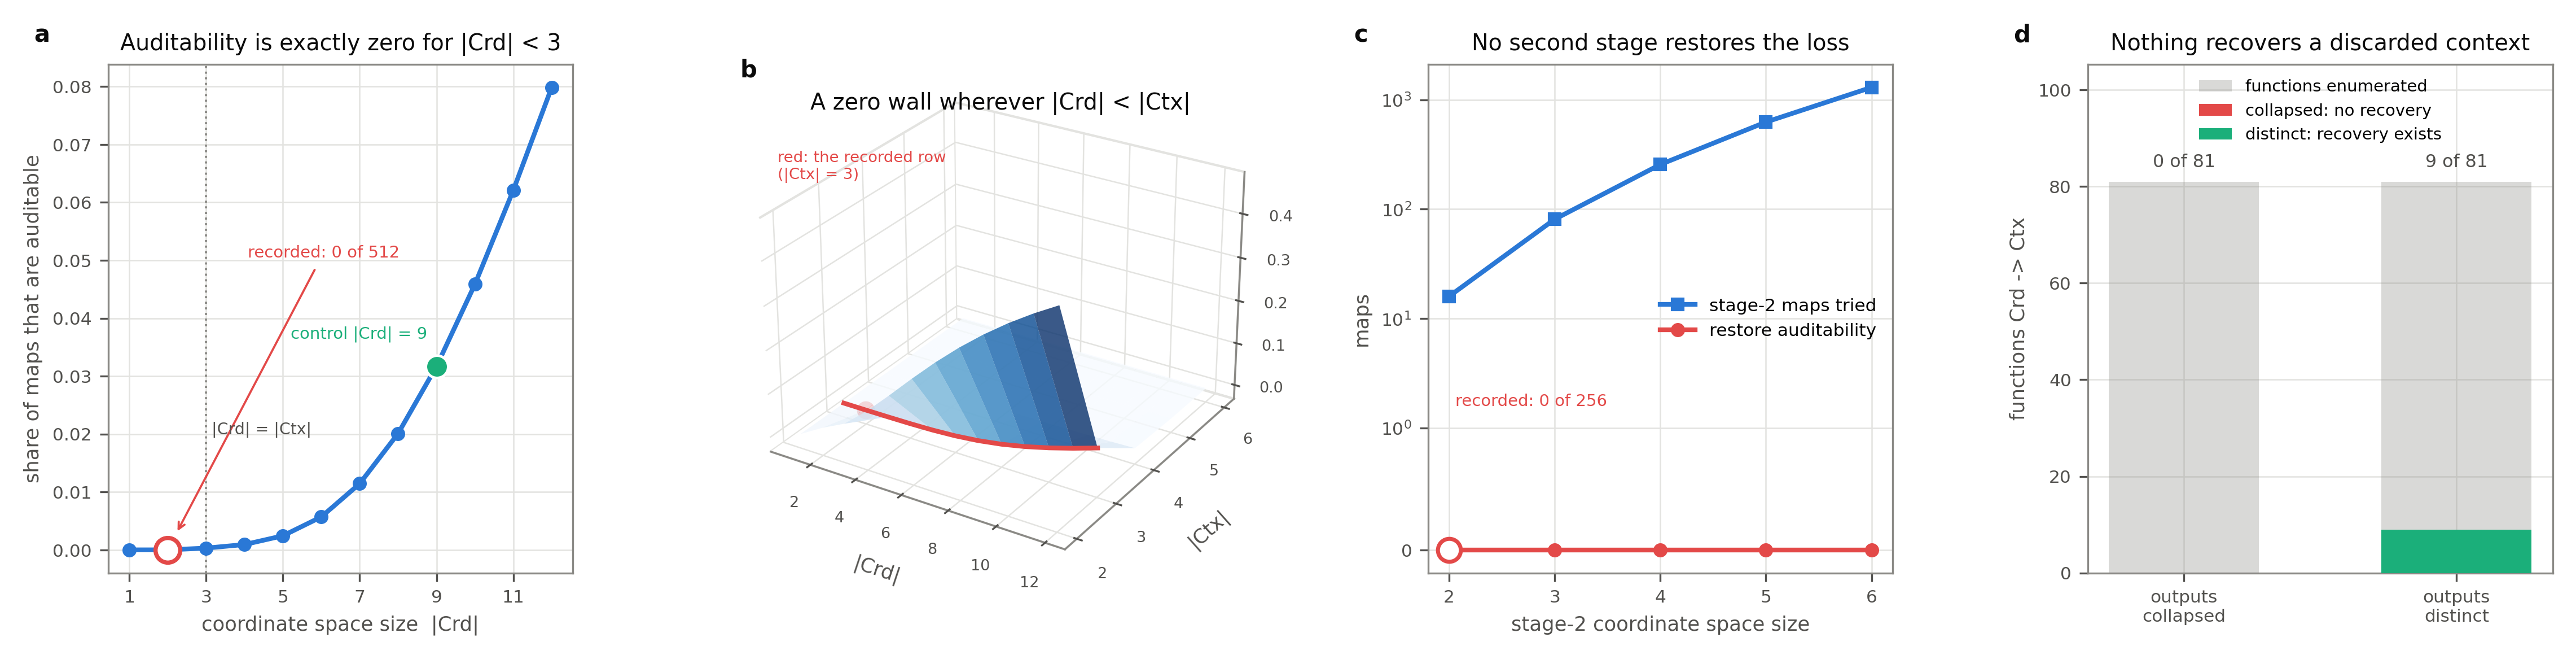
\includegraphics[width=\textwidth]{figures/panel1_collapse.png}
\caption{\Cref{thm:collapse}, \cref{thm:pipeline-loss} and
\cref{cor:no-recovery}. (a)~auditability against coordinate-space size,
which is exactly zero below $|\Ctx|$. (b)~the same over
$(|\Crd|, |\Ctx|)$: a zero wall wherever $|\Crd| < |\Ctx|$.
(c)~second stages attempted against auditability restored. (d)~candidate
recovery functions against contexts recovered.}
\label{fig:panel-collapse}
\end{figure}

\subsection{Collapse is forced by cardinality alone}

\Cref{thm:collapse} was graded against the observation that would refute
it --- an auditable coordinate map into a codomain smaller than the
context space. Over all $512$ maps from a $3$-element context space into
a $2$-element coordinate space, $0$ are auditable. The control matters:
widening the codomain to $9$ elements produces an auditable witness
immediately, so the zero is a consequence of the cardinality and not of
the enumeration being unable to recognise auditability.

\Cref{thm:pipeline-loss} was tested by asking whether the loss can be
undone downstream. Over all $256$ second stages, $0$ restored
auditability; the control confirms that composing an auditable first
stage with an injective second stage stays auditable, so the pipeline
machinery is not simply reporting failure everywhere.

\Cref{cor:no-recovery} is the sharpest of the three and was tested in
the strongest form available: the two pipeline outputs are checked to be
the \emph{same element}, and then all $81$ functions on that element are
enumerated. None recovers the context, which is what the corollary
asserts and is not an empirical claim about any particular estimator ---
it holds for every function, learned or otherwise. The control returns
$9$ successful recoveries as soon as the inputs are made distinct, which
is exactly the case \cref{rem:ml} says is not the one at issue.

\begin{figure}[htbp]
\centering
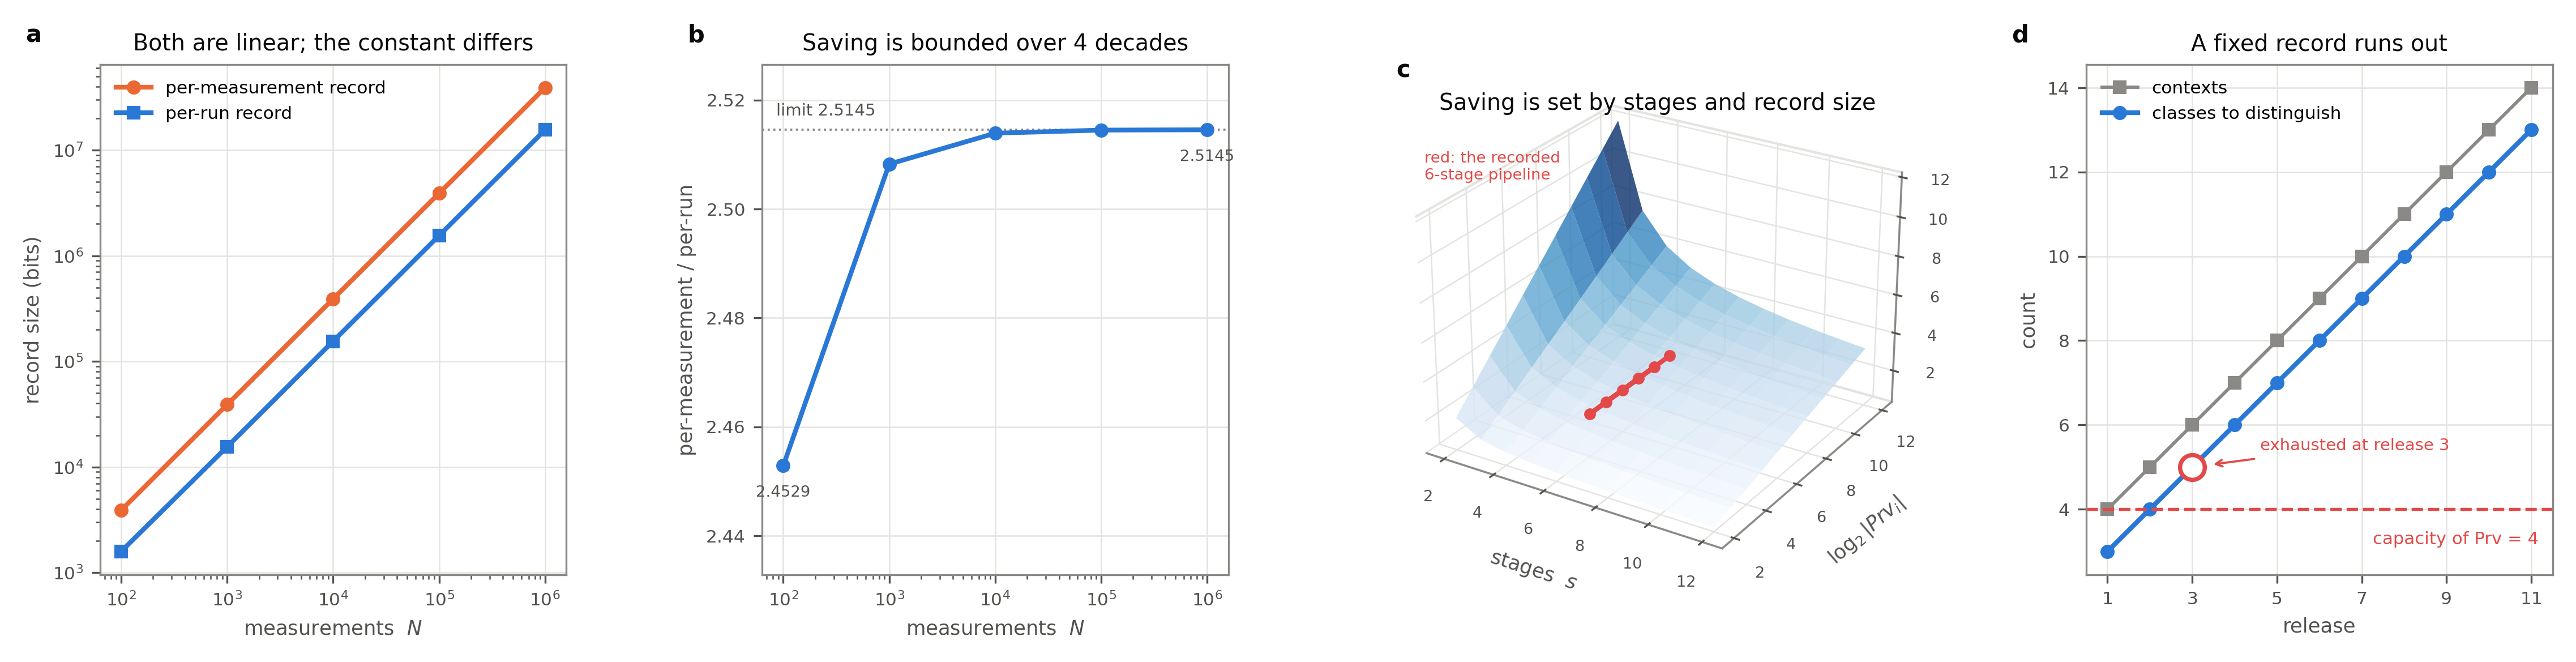
\includegraphics[width=\textwidth]{figures/panel2_record.png}
\caption{\Cref{prop:cost} and \cref{thm:record-floor}. (a)~cost of both
schemes against the number of measurements. (b)~the saving over five
decades of $N$. (c)~the saving over (stages, record size).
(d)~distinctions accumulating past a fixed record's capacity.}
\label{fig:panel-record}
\end{figure}

\subsection{The record is cheap, and the cost objection is quantitative}

\Cref{prop:cost} was graded against the observation that would sustain
the objection of \cref{rem:cost-reading}: a per-run scheme whose
advantage erodes as measurements accumulate. It does not erode. Over six
stages with record sizes $64, 128, 32, 256, 16, 512$, the per-run scheme
is cheaper at every $N$ tested, and the ratio is $2.4529$ at $N = 10^2$
and $2.5145$ at $N = 10^6$ --- flat to within $3\%$ over four decades.
The saving is bounded because the record is stored once per run rather
than amplified per measurement, which is the content of the proposition
rather than an artefact of the sizes chosen. The control makes the
dependence visible: with one very small stage the ratio reaches
$6884.1$, so the statistic is capable of moving by three orders of
magnitude and simply does not move with $N$.

\Cref{thm:record-floor} was tested against \cref{ax:noncomplete} by
running releases forward. A constant record is insufficient
immediately; a record of capacity $4$ is exhausted at release~$3$, where
$6$ contexts induce $5$ behavioural classes. The floor counts
distinctions rather than contexts, and the control shows the difference:
adding a context that is behaviourally a duplicate of an existing one
leaves the class count at $2$ and consumes no capacity.

\begin{figure}[htbp]
\centering
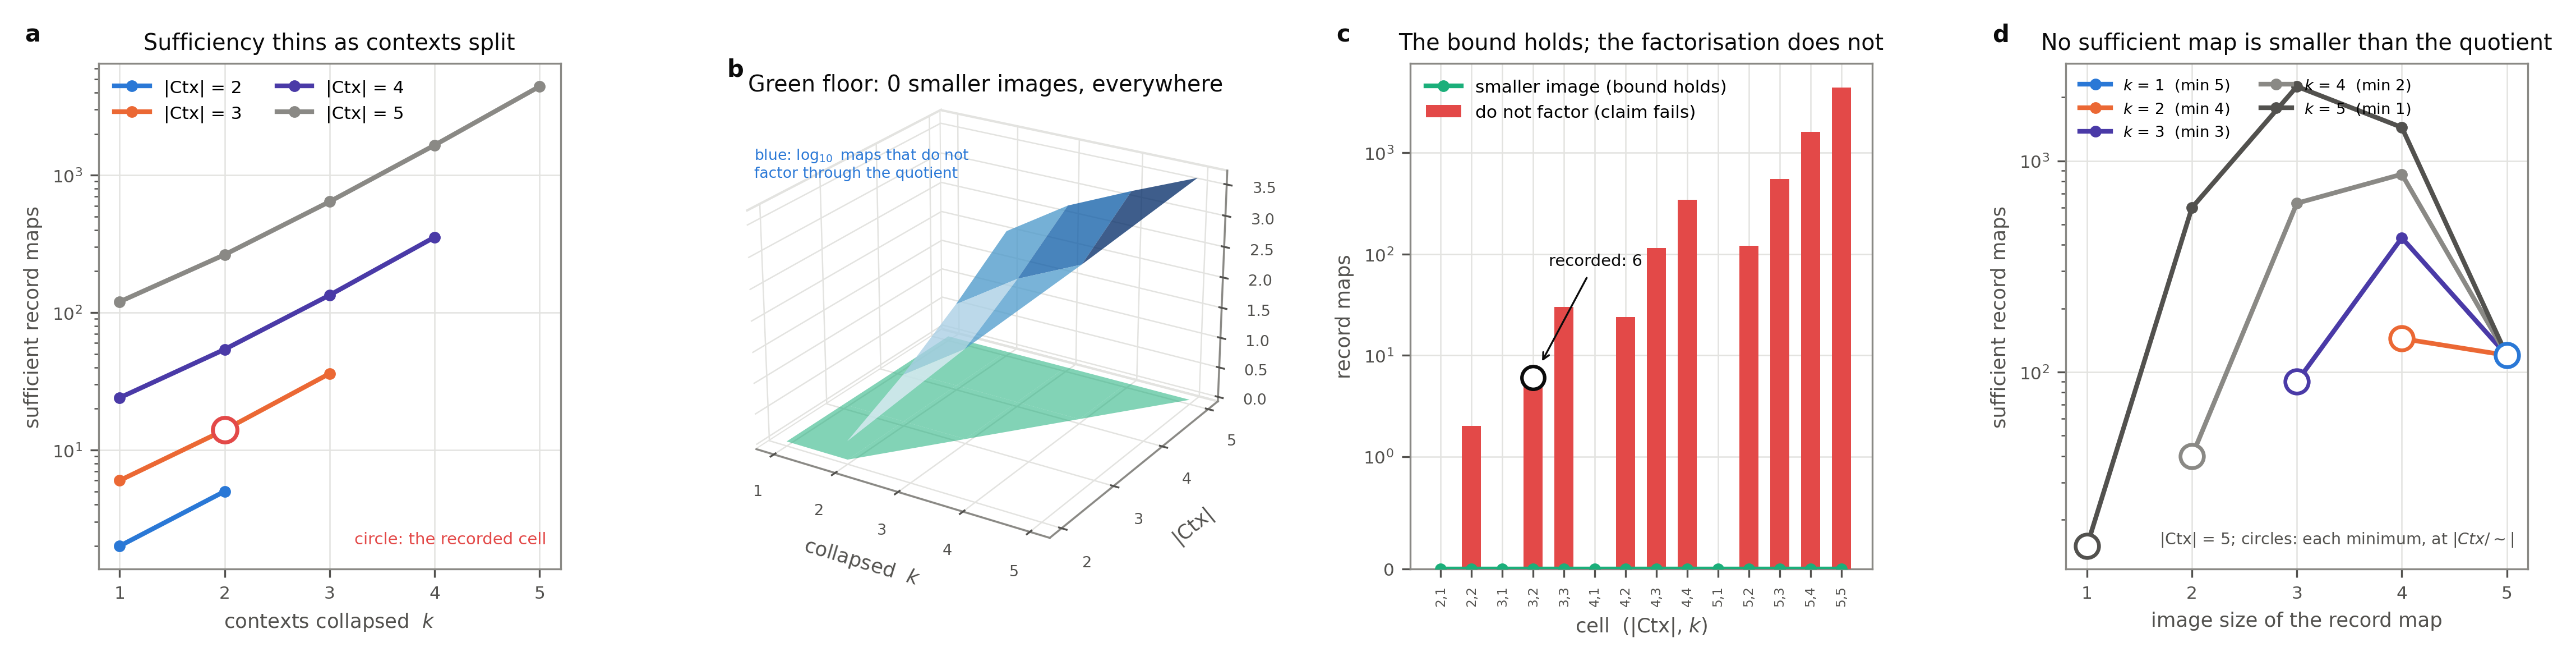
\includegraphics[width=\textwidth]{figures/panel3_minimality.png}
\caption{\Cref{thm:minimal-record}. (a)~sufficiency as contexts split.
(b)~the image-size floor over the parameter grid, zero everywhere.
(c)~the bound and the factorisation separated: the first holds, the
second does not. (d)~no sufficient map has an image smaller than the
behavioural quotient.}
\label{fig:panel-minimality}
\end{figure}

\subsection{A defect in \texorpdfstring{\cref{thm:minimal-record}}{Theorem: minimal record}}
\label{ssec:val-factorisation}

The theorem's bound reproduced exactly. With $3$ contexts falling into
$2$ behavioural classes, $\rec_{\min}$ is sufficient and $0$ sufficient
maps have a smaller image; the control confirms that smaller maps exist
and are simply not sufficient, so the minimum is a real one and not an
absence of candidates.

The theorem's \emph{proof}, however, asserts that every sufficient
record map factors through $\rec_{\min}$, and that is false. Six
sufficient maps do not factor through it. The counterexample is
immediate once stated: the map sending $c_1, c_2, c_3$ to $0, 1, 2$ is
sufficient --- it is injective, so it distinguishes everything a
sufficient map must --- yet it splits the class $\{c_1, c_2\}$ that
$\rec_{\min}$ identifies, and no map out of $\rec_{\min}$'s image can
recover that split. Sufficiency is closed upwards under refinement while
factorisation through the quotient requires coarseness, and the two
pull in opposite directions.

What survives is the statement the theorem is actually used for and
which its proof does establish: $\rec_{\min}$ attains the minimum image
size among sufficient maps, and is unique \emph{up to relabelling among
maps of that size}. The universal property should be struck from the
statement, or restricted to sufficient maps of minimal image. Nothing
elsewhere in the paper depends on the factorisation --- \cref{prop:cost}
uses the image size and \cref{thm:comparability} uses sufficiency ---
so the repair is local.

\begin{figure}[htbp]
\centering
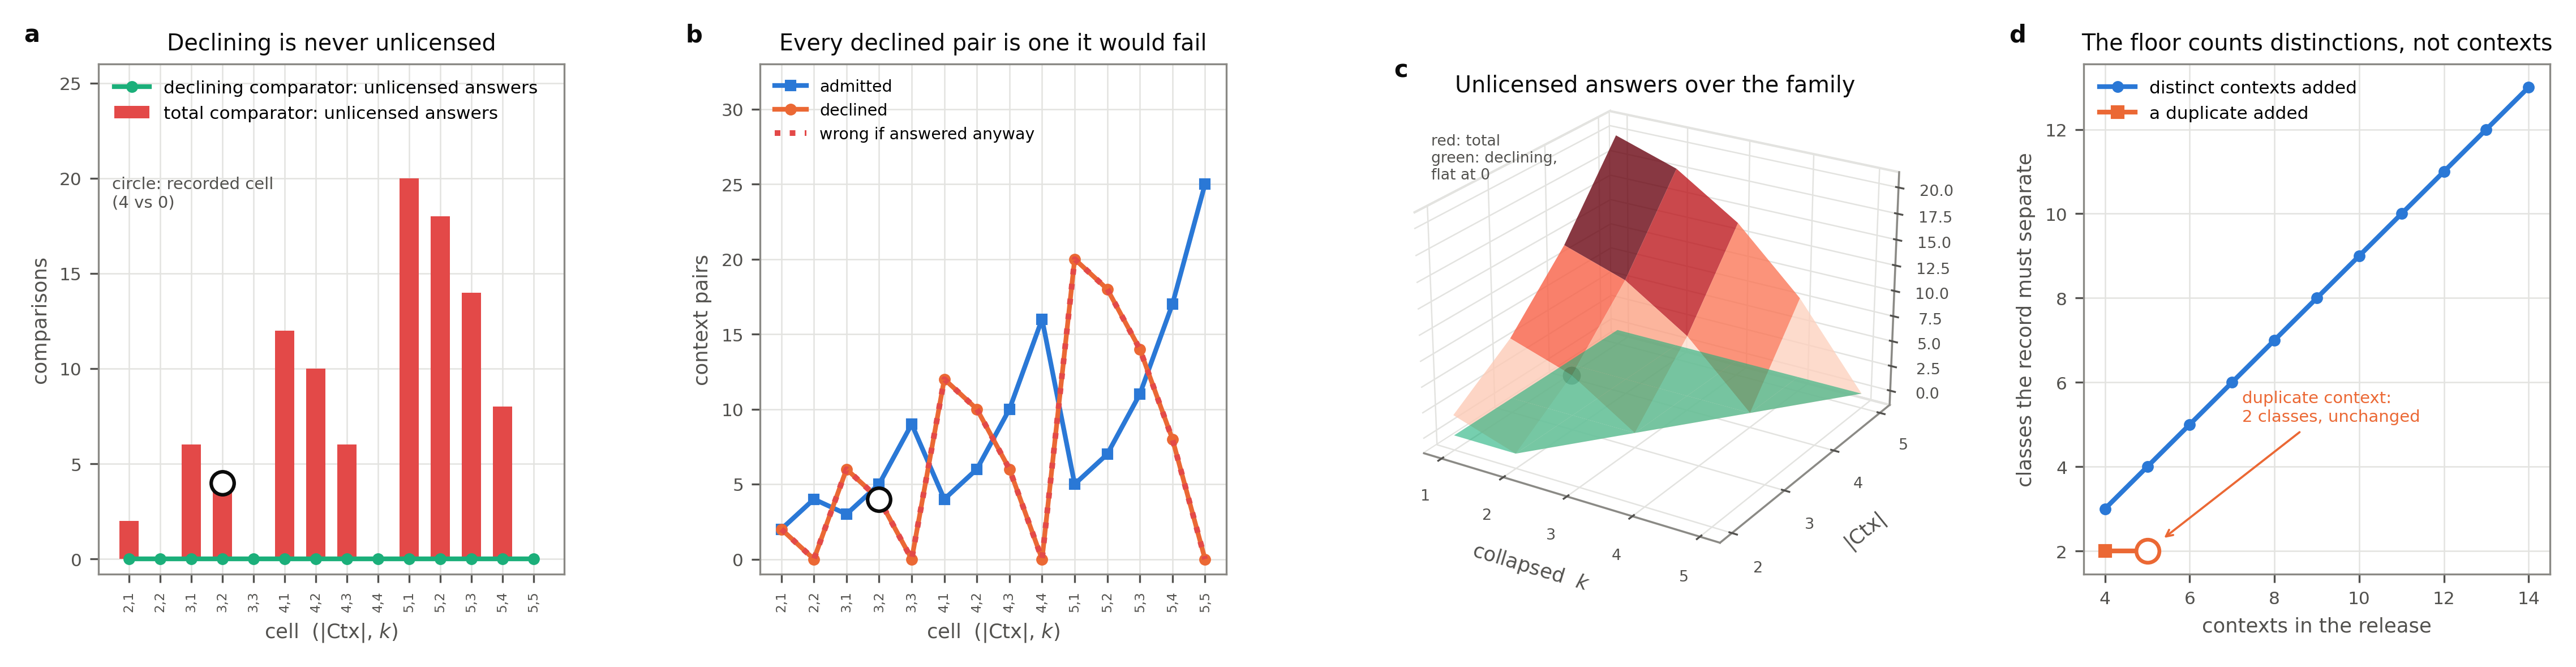
\includegraphics[width=\textwidth]{figures/panel4_declining.png}
\caption{\Cref{thm:comparability} and \cref{thm:decline-sound}.
(a)~admitted and declined comparisons against unsound admissions.
(b)~each declined pair against the answer a total comparator gives it.
(c)~unlicensed answers over the family of comparators. (d)~the floor as
a count of distinctions rather than of contexts.}
\label{fig:panel-declining}
\end{figure}

\subsection{Declining is sound, and a total comparator is not}

\Cref{thm:comparability} was graded against the observation that would
refute it --- an admitted comparison between measurements whose records
disagree. Of $45$ admitted pairs, $0$ are unsound. Four context pairs
were declined, so the comparator is not passing by admitting everything.

\Cref{thm:decline-sound} is the claim that the four declines are not a
weakness, and it was tested by putting a total comparator on the same
pairs. The total comparator answers $4$ unlicensed comparisons --- one
for each pair the partial comparator declines --- while the partial
comparator answers $0$ and declines all four. The counts coincide
exactly, which is the substance of \cref{rem:decline}: declining is not
a smaller answer than answering, it is the removal of precisely the
answers that are not licensed. A total comparator buys its totality by
being wrong on that set and nowhere else.

\subsection{What the validation does not establish}

The enumerations are exhaustive over small spaces --- three contexts,
two or nine coordinates, six stages --- which is what makes a reported
zero a proof rather than a search. It is not evidence about scale, and
none is claimed: \cref{thm:collapse} is a cardinality argument, so the
small case is the general case, whereas \cref{prop:cost}'s constant is a
property of the stage sizes supplied and would change with different
ones. What is measured there is that the constant does not grow with
$N$, which is the objection the proposition answers.
\Cref{ax:noncomplete} is an assumption about the world and is imposed
rather than tested; what is tested is what follows from it, namely that
a fixed record is exhausted at a definite release.

%======================================================================
\section{Discussion}
\label{sec:discussion}

\subsection{Relation to reproducibility practice}

Reporting guidelines require that acquisition and processing parameters
be published \citep{taylor2007guidelines}. This is necessary and is
addressed to a different problem: it lets a reader reconstruct what was
done. The results here concern what a pipeline may do with two numbers at
runtime, which is a question about types rather than about documentation.
A fully compliant publication can still contain an analysis that pooled
incomparable coordinates, because compliance records the contexts without
requiring the analysis to consult them.

\subsection{Relation to units and dimensional analysis}

Dimensional analysis is the special case in which $\Ctx$ is a set of unit
systems and the comparability rule is dimension matching. The results
here generalise it: contexts that are not unit choices --- library
version, reference channel, discretisation threshold --- obey the same
partiality discipline, and \Cref{thm:comparability} is the general form
of the rule that one may not add metres to seconds. The reason the
general case is neglected while the special case is universal is that
units are conventionally written next to the number, so the record is
carried by notation.

\subsection{Limitations}

\Cref{thm:minimal-record} characterises the minimal record up to
relabelling but does not give an algorithm for computing $\equiv$, which
would require deciding equality of the functions $\varphi(\cdot,c)$ on
all of $X$. In practice the equivalence is approximated by declaring
which fields of a configuration are behaviour-relevant, and an error in
that declaration produces exactly the unsound comparisons
\Cref{thm:decline-sound} is designed to exclude. \Cref{thm:comparability}
assumes the record map is sufficient; a pipeline whose record omits a
behaviour-relevant field satisfies the theorem's conclusion vacuously and
its guarantee not at all.

\subsection{Conclusion}

A derived coordinate is a function of a measurement and a context, the
coordinate space is smaller than the context-augmented domain, and so the
context is not recoverable from the coordinate. This is a counting fact,
not a deficiency of any particular pipeline, and it compounds along a
composition and is not repaired downstream. The remedy is to make the
coordinate a pair, to record exactly the distinctions that change the
map's behaviour, and to make comparison a partial operation that declines
on record mismatch. The cost is a pointer per measurement and a record
per run. The benefit is that comparisons the contexts do not license
become type errors rather than numbers.

% =====================================================================
\bibliographystyle{plainnat}
\bibliography{references}

\end{document}
